\documentclass[11pt, a4paper]{article}
\usepackage[style=script-v1, privacy=anonym]{../tools/library}
\renewcommand{\Lecturer}{Prof. A. Thom, Prof. V. Alekseev}


\begin{document}
\head{AL20: Algebra II}{Sommersemester 2026}

\tableofcontents

\newpage

\section{Reprise}

\subsection{Auswahlaxiom und das Zorn'sche Lemma}


\begin{note}
    Die Motivation dieses Rückblicks ist das Schaffen eines lückenlosen logischen Fundaments für das Studium unendlich-dimensionaler Vektorräume; Zumindest in der Hinsicht, dass bei der Konstruktion der Galoistheorie keine unangenehmen Widersprüche der Mengenlehre in die Quere kommen könnten.
\end{note}

\begin{lemma}[Linksinvertierbarkeit und Injektivität]
    Sei $X$ eine nichtleere Menge. Linksinvertierbare Abbildungen $i: X \to Y$ sind genau die injektiven Abbildungen. Heißt es gilt die Äquivalenz:
    $$i: X \to Y \text{ injektiv} \iff  \exists p: Y\to X: \ p\circ i=\id_X $$
    \begin{proof}[Beweisidee] \Rueck Für $x_1, x_2 \in X$ gilt $$i(x_1) = i(x_2) \yf p\circ i(x_1) = p\circ i(x_2) \yf x_1 = x_2$$
\Hin Da $i$ injektiv, ist $i: X \to i(X)$ eine Bijektion mit Umkehrabbildung $h: i(X) \to X$. Wähle
$$p: Y\longrightarrow X: y\longmapsto \begin{cases}
    h(y), \text{ falls } y\in i(X)\\
    x_0, \text{ sonst}
\end{cases}$$ 
für ein fest existierendes $x_0\in X\neq \leer$. Dann gilt $p\circ i= \id_X$
\end{proof}

\end{lemma}



\begin{note}[Rechtsinvertierbarkeit und Surjektivität]
    Tatsächlich gilt für eine endliche Menge $Y$ auch die duale Äquivalenz 
    $$\pi : X\to Y \text{ surjektiv} \iff \exists s: Y\to X: \ \pi \circ s= \id_Y$$
    \begin{proof}[Beweisidee]
        \Rueck Für $y\in Y$ gilt
        $$\pi(s(y)) = y \yf s(y) \in \pi\r (x)$$ 
        es existiert also zu jedem $y\in Y$ ein Urbild.
        \Hin Da $\pi$ surjektiv, wähle zu jedem $y\in Y$ ein $x_y \in \pi\r (y)$ und definiere
        $$s: Y\longrightarrow X: y\longmapsto x_y$$
        wohldefiniert, da $Y\neq \leer$. Dann gilt $\pi \circ s=\id_Y$
    \end{proof}
    Es stellt sich heraus, für eine unendliche Menge $Y$ ist das ">unendliche"< wählen im zweiten Teil nicht durch die klassischen Axiome der Mengenlehre gedeckt. Es braucht die folgende axiomatische Zusatzannahme:
\end{note}

\begin{definition}[Schnitt]\Theorem
    Sei $\pi : X\to Y$ eine surjektive Abbildung. Ein Rechtsinverses $s:Y\to X$ zu $\pi$ heißt Schnitt von $\pi$. 
\end{definition}
Wir postulieren:\bigskip

\phantomsection
\refstepcounter{subsubsection}
\addcontentsline{toc}{subsubsection}{Auswahlaxiom \arabic{section}.\arabic{subsection}.\arabic{subsubsection}}
\fbox{\textbf{Auswahlaxiom 1.1.5}} \textit{Jede surjektive Abbildung hat einen Schnitt.} \label{Auswahlaxiom}

\vspace{0.3cm}
\begin{definition}[Halbordnung]
    Sei $\Delta$ eine Menge. Eine Halbordnung auf $\Delta$ ist eine Relation $\preceq$ auf $\Delta$ mit folgenden Eigenschaften:
    \begin{itemize}
        \item[]  $\alpha \preceq \alpha$ für alle $\alpha \in \Delta$; \hfill (Reflexivität)
        \item[]  $\alpha \preceq \beta$ und $\beta \preceq \alpha \implies \alpha = \beta$ für $\alpha, \beta \in \Delta$; \hfill (Antisymmetrie)
        \item[] $\alpha \preceq \beta$ und $\beta \preceq \gamma \implies \alpha \preceq \gamma$ für $\alpha, \beta, \gamma \in \Delta$; \hfill (Transitivität) 
    \end{itemize}
    Eine Menge $\Delta$ mit einer festen Halbordnung $\preceq$ auf $\Delta$ heißt \emph{halbgeordnet}.
\end{definition}

\begin{definition}[Totalordnung] 
    Eine Halbordnung $\preceq$ auf einer Menge $I \subset \Delta$ heißt \emph{Totalordnung}, wenn
    $$x,y\in I \yf x\preceq y \text{ oder } y\preceq x$$
    Eine Menge $I\subset \Delta $ mit einer festen Totalordnung heißt \emph{Kette}.
\end{definition}

\begin{definition}[Obere Schranke und Maximalität]
    Sei $(\Delta, \preceq)$ eine halbgeordnete Menge und $I \subseteq \Delta$ eine Teilmenge. Ein Element $u \in \Delta$ heißt \emph{obere Schranke} für $I$, wenn für alle $i \in I$ gilt $i \preceq u$.\bigskip 
    
    Ein Element $m$ einer halbgeordneten Menge $(\Delta, \preceq)$ heißt \begin{enumerate}
        \item[] \emph{maximal}, wenn $ \forall x \in \Delta:\ m \preceq x \yf m = x$. 
        \item[]\emph{minimal}, wenn $\forall x \in \Delta: \ x \preceq m \yf m = x$.
    \end{enumerate}
\end{definition}

\begin{theorem}[Zorn'sches Lemma] \Theorem
    Sei $(\Delta, \preceq)$ eine halbgeordnete Menge mit der Eigenschaft, dass jede Kette $I \subseteq \Delta$ eine obere Schranke in $\Delta$ besitzt. Dann hat $\Delta$ ein maximales Element.
\end{theorem}

\begin{note}
    Es stellt sich heraus, dass das Zorn'sche Lemma nicht nur das Auswahlaxiom benötigt, sondern sogar zu ihm äquivalent ist. Statt des Auswahlaxioms in seiner Form \ref{Auswahlaxiom} könnte man also auch das Zorn'sche Lemma axiomatisch voraussetzen. Es folgen fundamentale Sätze
\end{note}

\begin{corollary}[Hamel] \Theorem Sei $\K$ ein Körper. Jeder $\K-$Vektorraum hat eine Basis.
\end{corollary}

\begin{corollary} Jeder $\K-$Vektorraum ist isomorph zu einer direkten Summe von Kopien von $\K$. Genauer, falls $\mathcal B$ Basis, dann 
$$V \xleftarrow{\cong}\bigoplus_{b\in \mathcal B} \K, \qquad \sum_{b\in \mathcal B} \lambda _b \cdot b \longmapsfrom \lambda_b$$
\end{corollary}

\begin{note}
    Äquivalent dazu ist übrigens: Jeder $\K-$Modul ist frei.
\end{note}

\begin{corollary}[Existenz eines Komplements]
    Sei $V$ ein Vektorraum und $U \subseteq V$ ein Untervektorraum. Dann gibt es einen Untervektorraum $W$ mit $V = U \oplus W$.
\end{corollary}

...und vieles mehr. Der gesamte restliche Inhalt dieses Manuskripts wird sich der Galoistheorie widmen, die diese Resultate nur noch implizit benötigen wird. Nichtsdestotrotz wird diese Reprise lohnenswert gewesen sein. Ein letzter Schluss, der aus dem Zorn'schen Lemma folgt, soll hier jedoch noch explizit erwähnt sein. Es ist nämlich dieser, auf welchem so ziemlich alles Nachfolgende aufbauen wird.

\begin{lemma}
    Sei $\K$ ein Körper und $f\in \K[t]$ irreduzibel. Dann ist der Quotient $\K[t]/(f)$ wieder ein Körper und kann insbesondere als Vektorraum über $\K$ verstanden werden. In diesem bilden für $d=\deg f$ die Polynomrestklassen
    $$[1], [t],\dots , [t^{d-1}]$$
    eine $\K$-Basis von $\K[t]/(f)$. Die Multiplikation mit dem Objekt $[t]$ wird durch die Begleitmatrix $\mathcal M_f\in \K^{d\times d}$ von $f$ beschrieben.
\end{lemma}


\newpage


\section{Allgemeine Körpererweiterungen}
\subsection{Grundlegende Begriffe und Erweiterung der Skalare}

\begin{definition}[Körpererweiterung] \Theorem
    Es seien $\L$ und $\K$ Körper, sodass $\K\subset \L$. Dann nennen wir $\L/\K$ eine Körpererweiterung.
\end{definition}

\begin{note}
    Das Studium der Galoistheorie wird sich hauptsächlich auf Körpererweiterungen einfacher algebraischer Art fokussieren. Was das bedeutet führen wir formal in \ref{Grad, Algebraisch, Transzendent} und \ref{Einfache Erweiterung} ein. Für jetzt wollen wir bemerken, dass falls wir eine Erweiterung $\L/\K$ mit $\K[t]/(f)$, also $\L$ als Vektorraum über $\K$, identifizieren können, dann verstehen wir die Struktur von $\L$ ziemlich gut. Einige Beispiele...
\end{note}

\begin{example} \label{ex: einfache Erweiterungen}\mbox{}
    \begin{enumerate}[label=(\roman*)]
        \item Für $\K = \R$ und $\L = \C$ ist $t^2+1 \in \R[t]$ irreduzibel und
        $$\C = \R(i) \cong \R[t]/(t^2+1).$$
        beide aufgefasst als $\R$-Vektorräume. Konkret entsteht die Isomorphie durch Basistransformation $(1,i) \longmapsto ([1],[t])$. Bezüglich der $\R$-Basis $(1,i)$ hat die Multiplikation mit $i$ die Matrix
        $$M_i = \begin{pmatrix} 0 & -1 \\ 1 & 0 \end{pmatrix}.$$
        Also wirkt jedes $a+bi \in \C$ durch
        $$aI_2 + bM_i = \begin{pmatrix} a & -b \\ b & a \end{pmatrix}.$$
        Das Minimalpolynom von $M_i$ ist $t^2+1$, und dieses zerfällt über $L = \C$ als $(t-i)(t+i)$ in paarweise verschiedene Linearfaktoren. Also ist $M_i$ über $L$ diagonalisierbar. Damit sind auch die Multiplikationsmatrizen aller Elemente von $L$, also aller Polynome in $M_i$, über $L$ diagonalisierbar.

        
        \item Für $\K = \Q$ und $\L = \Q(\sqrt2)$ ist $t^2-2$ irreduzibel und
        $$\Q(\sqrt2) \cong \Q[t]/(t^2-2).$$
        Wie in (i) haben die Multiplikationen mit $\sqrt2$ und $a+b\sqrt{2}$ bezüglich der Basis $(1,\sqrt2)$ die Matrizen
        $$M_{\sqrt2} = \begin{pmatrix} 0 & 2 \\ 1 & 0 \end{pmatrix} \qquad \& \qquad aI_2 + bM_{\sqrt2} = \begin{pmatrix} a & 2b \\ b & a \end{pmatrix}.$$
        Auch hier zerfällt $t^2-2$ über $\L$ in $(t-\sqrt2)(t+\sqrt2)$ paarweise verschiedene Linearfaktoren. Also ist auch diese Erzeugermatrix über $\L$ diagonalisierbar, und daher ebenso die Multiplikationsmatrix jedes Elements von $\L$.
        
        
        \item Für $\K = \Q$ und $\L = \Q(\sqrt[3]{2})$ ist $t^3-2$ irreduzibel und
        $$\Q(\sqrt[3]{2}) \cong \Q[t]/(t^3-2).$$
        Mit $\alpha = \sqrt[3]{2}$ und der Basis $(1,\alpha,\alpha^2)$ hat die Multiplikation mit $\alpha$ die Begleitmatrix
        $$M_\alpha = \begin{pmatrix} 0 & 0 & 2 \\ 1 & 0 & 0 \\ 0 & 1 & 0 \end{pmatrix}.$$
        Daher wirkt jedes $a+b\alpha+c\alpha^2$ durch
        $$aI_3 + bM_\alpha + cM_\alpha^2 = \begin{pmatrix} a & 2c & 2b \\ b & a & 2c \\ c & b & a \end{pmatrix}.$$
        Hier ist die Situation anders: das Minimalpolynom $t^3-2$ zerfällt über $\L$ nicht vollständig, weil die beiden anderen Nullstellen nicht in $\L$ liegen. Also ist die Erzeugermatrix $M_\alpha$ über $\L$ nicht diagonalisierbar. Insbesondere gibt es also bereits in $\L$ selbst Elemente, deren Multiplikationsmatrix über $\L$ nicht diagonalisierbar ist. Genau an diesem Punkt wird später der Unterschied zwischen den ersten zwei Beispielen und diesem Beispiel sichtbar.
    \end{enumerate}
\end{example}


\begin{note}
    An diesen Beispielen lässt sich das Prinzip einfacher Körpererweiterungen erkennen. Tritt $\L/\K$ als $\K(\alpha)/\K$ auf, so kommt diese Erweiterung verstanden als $\K$-Vektorraum mit einer Multiplikationsabbildung. Diese ist über $\K$ sicher nicht diagonalisierbar, aber aufgefasst als Matrix mit Einträgen in $\L$ können verschiedene Diagonalisierbarkeitsfälle eintreten. $\K$-lineare Abbildungen zu $\L$-linearen Abbildungen zu erweitern, ist auch die Motivation für die folgende Konstruktion.
\end{note}

\begin{lemma}[Erweiterung der Skalare für Vektorräume] \Theorem
 Sei $V$ ein $\K$-Vektorraum und $\K \subseteq \L$ eine Körpererweiterung. Betrachten wir $\L$ als einen $\K$-Vektorraum, so ist das Tensorprodukt
$$V_\L := V \otimes_\K \L$$
ein $\L$-Vektorraum bezüglich der Multiplikation (von rechts):
$$(v \otimes \mu)\lambda := v \otimes \mu \cdot \lambda$$
und es gilt $\dim_\L V_\L = \dim_\K V$. Wenn $f \in \Hom{V}{W}$, gilt: $$f_\L := f \otimes \id \in \Hom{V_\L}{W_\L}$$
Die Konstruktion von $V_\L$ aus $V$ (mit $\L$) nennt man eine \emph{Erweiterung der Skalare} von $\K$
zu $\L$ \end{lemma}

\begin{example} Wir haben einen natürlichen Isomorphismus 

$$M(m\times n, \K) \otimes_\K \L \cong M(m\times n, \L) \qquad \sum_{i=1}^k A_i \otimes \lambda_i \mapsto \sum_{i=1}^k \lambda_i A_i,$$
        insbesondere gilt $\K^n \otimes_\K \L \cong \L^n$. Das heißt, dass man den Übergang von $A$ gesehen als Matrix mit Einträgen in $\K$ zu $A$ als Matrix mit Einträgen in $\L$ genau als Erweiterung von Skalaren wahrnehmen kann.
\end{example}









\subsection{Algebraische \& Endliche Körpererweiterungen}

\begin{definition}[Grad, Algebraisch, Transzendent] \Theorem
    Sei $\L/\K$ eine Körpererweiterung.
    \begin{enumerate}[label=(\roman*)]
        \item Die Erweiterung $\L/\K$ heißt \emph{endlich}, wenn $\L$ als $\K$-Vektorraum endlichdimensional ist. In diesem Fall heißt
        $$[\L:\K] := \dim_\K(\L)$$
        der \emph{Grad} der Erweiterung.
        \item Ein Element $x \in \L$ heißt \emph{algebraisch} über $\K$, wenn es ein nichtkonstantes Polynom $f \in \K[t]$ gibt mit $f(x) = 0$.
        \item Ein Element $x \in \L$ heißt \emph{transzendent} über $\K$, wenn es nicht algebraisch über $\K$ ist.
        \item Die Erweiterung $\L/\K$ heißt \emph{algebraisch}, wenn jedes Element von $\L$ algebraisch über $\K$ ist.
        \item Für $x \in \L$ bezeichnen wir mit $\K(x)$ den kleinsten Teilkörper von $\L$, der $\K$ und $x$ enthält.
    \end{enumerate}
\end{definition}

\begin{mdbox}
\begin{lemma}[Endlichkeit gibt Algebraizität] \Theorem
    Jede endliche Körpererweiterung ist algebraisch.
\end{lemma}
\end{mdbox}

\begin{proof}[Beweisidee] Dieses Resultat scheint auf den ersten Blick algebraisch schwierig zu sein, ist es aber bei näherer Betrachtung überhaupt nicht. Bemerke nur, dass $[\L:\K]<\infty$ bedeutet, dass die Vektoren $1,x,\dots, x^{[\L:\K]}\in L$ linear abhängig sein müssen, also $a_0,\dots ,a_{[\L:\K]}\in \K$ nicht alle Null existieren, sodass $a_0+a_1x+\dots +a_{[\L:\K]}x^{[\L:\K]} = 0$
    
\end{proof}

\begin{lemma}[Minimalpolynom] \Theorem
    Sei $\L/\K$ eine Körpererweiterung und $x \in \L$ algebraisch über $\K$. Dann gibt es genau ein normiertes irreduzibles Polynom
    $$\mu_x = \mu_x^\K \in \K[t]$$
    mit $\mu_x(x) = 0$. Es teilt jedes Polynom $f \in \K[t]$ mit $f(x) = 0$. Dieses Polynom heißt das \emph{Minimalpolynom} von $x$ über $\K$.
    
    \begin{proof}[Beweisidee] Die Behauptung folgt ganz schnell aus der Tatsache, dass $\K[t]$ ein Hauptidealring ist und deshalb der Kern des Auswertungshomomorphismus $\ev_x : \K[t] \to \K$ ein solches Hauptideal sein muss; erzeugt von einem minimalen Element $\mu_x$.
\end{proof}

\end{lemma}



\begin{lemma}[Gradformel] \Theorem Sei $\L/\K$ eine Körpererweiterung und $x \in \L$ algebraisch über $\K$. Dann ist die Abbildung
    $$\K[t]/(\mu_x) \xrightarrow{\Phi} \K(x), \quad [f(t)] \mapsto f(x)$$
    ein Isomorphismus von $\K$-Algebren. Insbesondere gilt
    $$[\K(x):\K] = \deg(\mu_x).$$
\end{lemma}

\begin{note}
    Surjektivität folgt daraus, dass $\K(x)$ als $\K$-Algebra gerade von $x$ erzeugt wird. Der Kern ist gerade $(\mu_x)$, also induziert der Quotient einen Isomorphismus.
\end{note}

\begin{theorem}[Turmformel] \Theorem
    Seien $\K \subseteq \E \subseteq \L$ Körper und seien $\E/\K$ und $\L/\E$ endlich. Dann ist auch $\L/\K$ endlich und es gilt
    $$[\L:\K] = [\L:\E]\,[\E:\K].$$
\end{theorem}


\begin{definition}[Zerfällungskörper] \Theorem
    Sei $\K$ ein Körper und $0 \neq f \in \K[t]$. Ein Körper $\L \supseteq \K$ heißt \emph{Zerfällungskörper} von $f$ über $\K$, wenn
    \begin{enumerate}[label=(\roman*)]
        \item das Polynom $f$ in $\L[t]$ in Linearfaktoren zerfällt und
        \item $\L$ von den Nullstellen von $f$ über $\K$ erzeugt wird.
    \end{enumerate}
\end{definition}


\begin{theorem}[Existenz und Endlichkeit des Zerfällungskörpers] \Theorem
    Zu jedem nichtkonstanten Polynom $f \in \K[t]$ existiert ein Zerfällungskörper $\L \supseteq\K$. Diese Körpererweiterung $\L/\K$ ist endlich.
\end{theorem}

\begin{theorem}[Eindeutigkeit bis auf Isomorphie]
    Sei $f \in \K[t]$. Sind $\L$ und $\L'$ Zerfällungskörper von $f$ über $\K$, so gibt es einen $\K$-Isomorphismus
    $$\tilde\varphi: \L \to \L'.$$
\end{theorem}

\begin{definition}[Algebraischer Abschluss] \Theorem
    Ein \emph{algebraischer Abschluss} eines Körpers $\K$ ist eine algebraische Körpererweiterung $\L/\K$, wobei $\L$ algebraisch abgeschlossen ist; Jedes nichtkonstante Polynom in $\K[t]$ zerfällt bereits vollständig in Linearfaktoren über $\L$
\end{definition}

\begin{theorem}
    Jeder Körper besitzt einen algebraischen Abschluss. Zwei algebraische Abschlüsse sind über den Grundkörper isomorph.
\end{theorem}


\begin{note}
    Wir bezeichnen mit $\overline\K$ den algebraischen Abschluss von $\K$. Ist $\L$ algebraisch abgeschlossen und $\K\subset \L$, dann gibt es eine natürliche Einbettung $\overline{\K}\hookrightarrow\L$. Beispiel: $\overline \Q \hookrightarrow \C$
\end{note}

\newpage
\section{Galoiserweiterungen}

\subsection{Multiplikationsendomorphismen}
Es sei stets $\L/\K$ eine endliche Körpererweiterung. Betrachte $\L\otimes _\K \L$ als $\L$-Algebra mit skalarer Multiplikation über dem zweiten Faktor.
$$a\cdot(x\otimes_\K y)= x\otimes_\K ay$$


\begin{lemma}[Erweiterung der Skalare für Körper] \Theorem
    Sei \ $\L/\K$ eine Körpererweiterung, $x$ algebraisch über $\K$, und $\mu_x \in \K[t]$ das Minimalpolynom von $x$ über $\K$. Dann ist die Abbildung
    $$\L[t] \to \K(x) \otimes_\K \L, \quad f(t) \mapsto f(x\otimes 1)$$
    surjektiv, und ihr Kern ist das von $\mu_x$ erzeugte Ideal. Insbesondere gibt es einen natürlichen Isomorphismus von $\L$-Algebren
    $$\K(x) \otimes_\K \L \cong \L[t]/(\mu_x).$$
\end{lemma}

\begin{note}
    Dieses Lemma ist unsere formale Rechtfertigung dafür, die Multiplikationsabbildungen in \ref{ex: einfache Erweiterungen} mit Koeffizienten in $\K$ nun als lineare Operatoren mit Koeffizienten in $\L$ aufzufassen. Es beweist, dass durch Hinzunahme von mehr ">Darstellungsmöglichkeiten<" keine Struktur verloren geht. Möglicherweise stehen dann für die Diagonalisierbarkeit über $\L$ ">genug"< Zahlen zur Verfügung. Wir können das sogar noch konkretisieren:
\end{note}

\begin{lemma}[Begleitmatrix der Multiplikation] \Theorem
    Sei $x \in \L$, und setze
    $\E := \K(x), \ d := [\E:\K]$.
    Sei $\mu_x$ das Minimalpolynom von $x$ über $\K$, und sei $C_{\mu_x}$ die Begleitmatrix
    $$\mu_x(t) = t^d + c_{d-1}t^{d-1} + \cdots + c_0\qquad C_{\mu_x} = \begin{pmatrix}
        0 & 0 & \cdots & 0 & -c_0 \\
        1 & 0 & \cdots & 0 & -c_1 \\
        0 & 1 & \cdots & 0 & -c_2 \\
        \vdots & \vdots & \ddots & \vdots & \vdots \\
        0 & 0 & \cdots & 1 & -c_{d-1}
    \end{pmatrix}  $$
    Dann hat der Endomorphismus
    $$m_x: \E\otimes_\K \L \to \E\otimes_\K \L, \quad z \mapsto (x\otimes 1)z$$
    bezüglich der $\L$-Basis
    $(1\otimes 1,\ x\otimes 1,\ \dots,\ x^{d-1}\otimes 1)$
    die Matrix $C_{\mu_x}$.
\end{lemma}

Nun können wir daran ganz praktisch Diagonalisierbarkeitsfälle charakterisieren

\begin{corollary} 
    Sei $x \in \L$. Dann sind jeweils äquivalent:\\
    
    \begin{center}
    \begin{minipage}[c]{0.42\textwidth}\raggedleft
        $\mu_x$ zerfällt in $\L[t]$ in Linearfaktoren
    \end{minipage}
    \hfill $\iff$ \hfill
    \begin{minipage}[c]{0.42\textwidth}\raggedright
        $\chi_{m_x}$ zerfällt in $\L[t]$ in Linearfaktoren
    \end{minipage}

    \vspace{0.4cm}

    \begin{minipage}[c]{0.42\textwidth}\raggedleft
        $\mu_x$ hat keine mehrfachen irreduziblen Faktoren
    \end{minipage}
    \hfill $\iff$ \hfill
    \begin{minipage}[c]{0.42\textwidth}\raggedright
        $\mu_x$ hat in seinem Zerfällungskörper keine mehrfache Nullstelle
    \end{minipage}

    \vspace{0.4cm}

    \begin{minipage}[c]{0.42\textwidth}\raggedleft
        $m_x$ ist über $\L$ diagonalisierbar
    \end{minipage}
    \hfill $\iff$ \hfill
    \begin{minipage}[c]{0.42\textwidth}\raggedright
        $\mu_x$ zerfällt in $\L[t]$ in paarweise verschiedene Linearfaktoren
    \end{minipage}
    \end{center}
\end{corollary}


\begin{definition}[Normal, Separabel, Galois] \Theorem
    Sei $\K \subseteq \L$ eine Körpererweiterung.
    \begin{enumerate}[label=(\roman*)]
        \item Das Element $x \in \L$ heißt \emph{normal} über $\K$, wenn $\mu_x$ über $\L$ in Linearfaktoren zerfällt.
        \item Das Element $x \in \L$ heißt \emph{separabel} über $\K$, wenn $\mu_x$ keine mehrfachen irreduziblen Faktoren hat.
        \item Das Element $x \in \L$ heißt \emph{Galois} über $\K$, wenn $m_x$ über $\L$ diagonalisierbar ist.
    \end{enumerate}
 Entsprechend heißt die Körpererweiterung  $\L/\K$ normal / separabel / Galois, wenn alle $x\in \L$ normal / separabel / Galois über $\K$ sind.
\end{definition}

\begin{example}[zu \ref{ex: einfache Erweiterungen}]  \label{ex: normal, separabel, Galois} \mbox{}
    \begin{enumerate}[label=(\roman*)]
        \item ist Galois, da $\mu_x$ in paarweise verschiedene Linearfaktoren zerfällt. Also auch das Minimalpolynom von $a+bi$.
        \item ist Galois aus demselben Grund.
        \item ist separabel aber nicht normal.
        \item Wir wollen uns auch ein Beispiel für eine normale, nicht separable Körpererweiterung überlegen. Nimm 
        $$\K= \F_p (t) = \left\{\frac{f}{g}\; \Big| \; f,g\in \F_p[t], g\neq 0\right\}$$
        den rationalen Funktionenkörper über $\F_p$. Betrachte nun das Polynom $f(x) = x^p - t \in \K[x]$, dies ist irreduzibel über $\K$. ($t$ ist keine $p$-te Potenz in $\F_p(t)$.) Sei $\alpha\in \ker f$ und $\L=\K(\alpha).$ Dann ist  $\mu_\alpha = x^p-t$ das Minimalpolynom von $\alpha$, doch über $\L[x]$ gilt 
        $$x^p -t = (x-\alpha)^p$$
        Also zerfällt $f\in \L[x]$ in Linearfaktoren mit $p$-facher Nullstelle.
        
    \end{enumerate}
\end{example}

\subsection{Separabilität}

\begin{note}In \ref{ex: normal, separabel, Galois} fällt bereits auf, dass (Nicht-)Separabilität eine weitaus ">mysteriösere"< Eigenschaft als Normalität ist. Wir wollen daher separable Polynome spezifischer charakterisieren. 
\end{note}

\begin{definition}[Formale Ableitung]
    Sei $\K$ ein Körper und
    $$f(t) = a_0 + a_1t + \cdots + a_nt^n \in \K[t].$$
    Dann heißt
    $$f'(t) := a_1 + 2a_2t + \cdots + na_nt^{n-1}$$
    die \emph{formale Ableitung} von $f$.
\end{definition}

\begin{lemma}
    Sei $\K$ ein Körper, $f \in \K[t]$, $\L/\K$ eine Körpererweiterung und $\alpha \in \L$. Dann sind äquivalent:
    \begin{enumerate}[label=(\roman*)]
        \item $\alpha$ ist eine mehrfache Nullstelle von $f$, d.h. $(t-\alpha)^2$ teilt $f$ in $\L[t]$.
        \item Es gilt $f(\alpha) = 0$ und $f'(\alpha) = 0.$
    \end{enumerate}
\end{lemma}

\begin{lemma}
    Sei $\K$ ein Körper und $\Char \K = 0$; sei $x$ algebraisch über $\K$. Dann hat $\mu_x$ in seinem Zerfällungskörper keine mehrfache Nullstelle.
\end{lemma}

\begin{mdbox}
\begin{corollary}[Endlichkeit in char 0 gibt Separabilität] \Theorem
    Jede endliche Körpererweiterung $\L/\K$ mit $\mathrm{char}(\K) = 0$ ist separabel.
\end{corollary}
\end{mdbox}

\begin{definition}[Separabilität, Allgemein] \Theorem
    Sei $\K$ ein Körper und $0 \neq f \in \K[t]$. Das Polynom $f$ heißt \emph{separabel}, wenn es in seinem Zerfällungskörper keine mehrfache Nullstelle besitzt.
\end{definition}

\begin{lemma}[Ableitungskriterium] \Theorem
    Sei $\F$ ein Körper und $0 \neq f \in \F[t]$. Dann sind äquivalent:
    \begin{enumerate}[label=(\roman*)]
        \item $f$ ist separabel.
        \item $\gcd(f,f') = 1$.
        \item Für jede Körpererweiterung $\E/\F$ tritt in der Faktorisierung von $f$ in $\E[t]$ in irreduzible Polynome kein Faktor mehrfach auf.
    \end{enumerate}
\end{lemma}

\begin{corollary}
    Sei $\E/\F$ eine Körpererweiterung und sei $f \in \F[t]$ separabel. Dann ist $f$, als Element von $\E[t]$ aufgefasst, ebenfalls separabel.
\end{corollary}

\begin{lemma} \label{lm: charakterisierung nicht separabilität}
    Sei $\F$ ein Körper der Charakteristik $p>0$, und sei $f \in \F[t]$ irreduzibel. Dann sind äquivalent:
    \begin{enumerate}[label=(\roman*)]
        \item $f$ ist nicht separabel.
        \item $f'(t) = 0$.
        \item Es gibt ein irreduzibles Polynom $g \in \F[t]$ mit
        $$f(t) = g(t^p).$$
    \end{enumerate}
\end{lemma}

\begin{definition}[Perfekter Körper] \Theorem
    Ein Körper $\K$ heißt \emph{perfekt}, wenn jedes irreduzible Polynom $f\in \K[t]$ separabel ist. (Oder äquivalent: Jede algebraische Erweiterung von $\K$ ist separabel.)
\end{definition}

\begin{mdbox}
\begin{theorem}[über Perfekte Körper]\label{über Perfekte Körper}
    Sei $\K$ ein Körper. Ist $\Char \K = 0$ oder $|\K|<\infty$, dann ist $\K$ perfekt.
\end{theorem}
\end{mdbox}

\begin{proof}[Beweisidee] Für $\Char \K = 0$ wähle man $f\in \K[t]$ irreduzibel. Dann ist $\K[t]/(f)$ eine endliche Körpererweiterung. Nach \ref{Endlichkeit in char 0 gibt Separabilität} ist diese separabel. Also ist $f$ separabel über $\K$. Für $|\K|<\infty$ gilt gleich $\Char \K = p$ und es gibt den Frobenius-Automorphismus $\Phi: \F_p \to \F_p, x\mapsto x^p$. Dieser führt die Annahme $f\in \F_p[t]$ irreduzibel und nicht separabel zum Widerspruch, da kein irreduzibles $g\in \F_p[t]$ mit $f(t)=g(t^p)$ existieren kann (siehe \ref{lm: charakterisierung nicht separabilität}).
\end{proof}

\newpage


\begin{definition}[Einfache Erweiterung] \label{Einfache Erweiterung}
Eine Körpererweiterung $\L/\K$ heißt einfach, falls $\L = \K(\alpha)$ für ein $\alpha\in \L$.
\end{definition}

\begin{mdbox}
\begin{theorem}[vom Primitiven Element] \Theorem
    Jede endliche separable Körpererweiterung $\L/\K$ ist einfach. 
\end{theorem}
\end{mdbox}

Mit einiger Arbeit mehr in der Ringtheorie, kann man außerdem zeigen:

\begin{corollary}[Transitivität der Separabilität]
    Seien $\K \subseteq \E \subseteq \L$ endliche Körpererweiterungen. Sind $\E/\K$ und $\L/\E$ separabel, so ist auch $\L/\K$ separabel.
\end{corollary}


\subsection{Körperautomorphismen}

\begin{note}
    Unter den Ringhomomorphismen gibt es eben auch die noch spezielleren $\K$-Algebren-Homomorphismen, die zusätzlich mit skalarer Multiplikation verträglich sind. Wir untersuchen den Vektorraum $\mathrm{Hom}_\K(\L,\F)$ dieser Homomorphismen zwischen zwei $\K$-Algebren und stellen Erstaunliches fest
\end{note}

\begin{lemma}[Artin] \Theorem
    Seien $\L/\K$ eine Körpererweiterung, $\F$ ein Körper und
    $$\sigma_1, \dots, \sigma_r: \L \to F$$
    paarweise verschiedene $\K$-Algebrenhomomorphismen. Dann sind $\sigma_1,\dots,\sigma_r$ $\F$-linear unabhängig (als Abbildungen $\L\to \F$). Also für $a_1,\dots , a_r\in \F$
    $$a_1\sigma_1+\dots +a_r\sigma_r = 0 \iff a_1,\dots , a_r=0 $$
\end{lemma}

\begin{definition}[Automorphismengruppe] \Theorem
    Sei $\L/\K$ eine Körpererweiterung. Die Automorphismengruppe von $\L/\K$ ist definiert als
    $$\mathrm{Aut}(\L/\K) = \{\sigma \in \mathrm{Aut}(\L) \mid \sigma|_\K = \id_\K\}$$
    (hierbei ist $\mathrm{Aut}(\L)$ die Automorphismengruppe von $\L$ als Ring, also die Gruppe aller Ringisomorphismen $\L \to \L$).
\end{definition}

\begin{corollary}
    Für jede endliche Körpererweiterung $\L/\K$ gilt
    $$|\mathrm{Aut}(\L/\K)| \leq [\L:\K].$$
\end{corollary}


\begin{definition}[Galoisgruppe] \Theorem
    Ist $\L/\K$ eine Galois-Erweiterung, so heißt
    $$\mathrm{Gal}(\L/\K) := \mathrm{Aut}(\L/\K)$$
    die \emph{Galoisgruppe} von $\L/\K$.
\end{definition}

\begin{theorem}[Galois-Charakterisierung durch Aut(L/K)] \Theorem
    Für eine endliche Erweiterung $\L/\K$ sind äquivalent:
    \begin{enumerate}[label=(\roman*)]
        \item $\L/\K$ ist eine Galois-Erweiterung.
        \item Es gilt
        $|\mathrm{Aut}(\L/\K)| = [\L:\K].$
        \item Es gibt einen $\L$-Algebrenisomorphismus
        $\L \otimes_\K \L \cong \L^{[\L:\K]}.$
    \end{enumerate}
\end{theorem}

\begin{lemma}
    Sei $V$ ein endlichdimensionaler $\K$-Vektorraum, und seien $f_1,\dots,f_n \in \End{V}$ paarweise kommutierende diagonalisierbare Endomorphismen. Dann gibt es eine Basis von $V$, bezüglich der alle $f_i$ diagonal sind.
\end{lemma}


\begin{theorem}[Galois-Charakterisierung durch Zerfällungskörper] \Theorem
    Für eine endliche Erweiterung $\L/\K$ sind äquivalent:
    \begin{enumerate}[label=(\roman*)]
        \item $\L/\K$ ist eine Galois-Erweiterung.
        \item Es gibt ein separables Polynom $f \in \K[t]$, dessen Zerfällungskörper über $\K$ gleich $\L$ ist.
        \item Es gibt ein irreduzibles separables Polynom $p \in \K[t]$, dessen Zerfällungskörper über $\K$ gleich $\L$ ist.
    \end{enumerate}
\end{theorem}

\begin{corollary}[Transitivität auf Nullstellen]
    Sei $\L/\K$ eine endliche Galois-Erweiterung. Wählt man ein primitives Element $\alpha \in \L$, so ist $\L$ der Zerfällungskörper des separablen irreduziblen Polynoms $\mu_\alpha$, und $\mathrm{Gal}(\L/\K)$ wirkt transitiv auf der Menge seiner Nullstellen in $\L$.
\end{corollary}



\begin{corollary}
    Sei $\L/\K$ eine endliche separable Erweiterung. Dann gibt es eine endliche Galois-Erweiterung $\M/\K$ mit $\L \subseteq \M$.
\end{corollary}

\newpage

\subsection{Galoiskorrespondenz}

\begin{definition}[Fixkörper]
    Sei $\L/\K$ eine Galois-Erweiterung mit Galoisgruppe
    $$G := \mathrm{Gal}(\L/\K).$$
    \begin{enumerate}[label=(\roman*)]
        \item Ist $H \leqslant G$ eine Untergruppe, so heißt
        $$\L^H := \{x \in \L \mid \sigma(x) = x \text{ für alle } \sigma \in H\}$$
        der \emph{Fixkörper} von $H$.
        \item Ist umgekehrt $\K \subseteq \E \subseteq \L$ ein Zwischenkörper, so setzen wir
        $$\mathrm{Aut}(\L/\E) := \{\sigma \in G \mid \sigma|_\E = \id_\E\}$$
    \end{enumerate}
\end{definition}

\begin{theorem}[Hauptsatz der Galoistheorie] \Theorem
    Sei $\L/\K$ eine endliche Galois-Erweiterung und
    $$G := \mathrm{Gal}(\L/\K).$$
    Dann ist die folgende Zuordnung
    \begin{align*}
    \E &\xmapsto{\qquad\qquad} \Aut{\L/\E} \\
    \left\{\E\;\Big| \; \K\subseteq \E\subseteq \L\right\}& \mathrel{\substack{\xrightarrow[]{\qquad\qquad} \\ \substack{\xleftarrow[]{\qquad\qquad}}}}\left\{H\;\Big|\; H\leqslant G\right\}\\
    \L^H & \xmapsfrom{\qquad \qquad} H
    \end{align*}
    eine inklusionsumkehrende \emph{Bijektion} von Zwischenkörpern $\K\subseteq \E\subseteq \L$ und Untergruppen $H\leqslant G$ Außerdem gilt:
    \begin{enumerate}[label=(\roman*)]
        \item Für jeden Zwischenkörper $\E$ gilt
        $$[\L:\E] = |\mathrm{Aut}(\L/\E)| \qquad \text{und} \qquad [\E:\K] = [G:\mathrm{Aut}(\L/\E)].$$
        \item Für jede Untergruppe $H \leqslant G$ gilt
        $$[\L:\L^H] = |H| \qquad \text{und} \qquad [\L^H:\K] = [G:H].$$
        \item Für einen Zwischenkörper $\E$ sind äquivalent:
        \begin{enumerate}[label=(\alph*)]
            \item $\E/\K$ ist eine Galois-Erweiterung.
            \item $\mathrm{Aut}(\L/\E) \triangleleft G$.
        \end{enumerate}
        In diesem Fall induziert die Einschränkung einen Isomorphismus
        $$G/\mathrm{Aut}(\L/\E) \cong \mathrm{Gal}(\E/\K).$$
    \end{enumerate}
\end{theorem}


\newpage
\section{Abelsche\hspace{6pt}\& Radikalerweiterungen}


Zunächst wollen wir uns an einige Definitionen und Resultate über abelsche und auflösbare Gruppen aus Algebra I erinnern.


\subsection{Abelianisierung und Auflösbarkeit}

\begin{definition}[Abelianisierung]
\Theorem
Ist $G$ eine Gruppe, so bezeichnen wir mit $[G,G]$ die von allen Kommutatoren
\[
[g,h] = ghg^{-1}h^{-1} \quad (g,h \in G)
\]
erzeugte Untergruppe. Dann ist $[G,G] \trianglelefteq G$, und der Quotient
\[
G^{\mathrm{ab}} := G/[G,G]
\]
ist abelsch. Er heißt die \emph{Abelianisierung} von $G$.
\end{definition}

\begin{lemma}[Universelle Eigenschaft der Abelianisierung] \label{Universelle Eigenschaft der Abelianisierung}
Sei $G$ eine Gruppe. Dann ist $G/[G,G]$ abelsch. Ist $A$ eine abelsche Gruppe und $\varphi : G \to A$ ein Gruppenhomomorphismus, so gibt es genau einen Homomorphismus $\overline{\varphi}: G/[G,G]\to A$, der das Dreieck kommutieren lässt

\begin{figure}[h]
    \centering
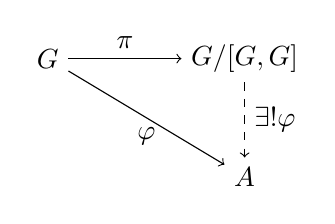
\begin{tikzpicture}[node distance=1cm, auto]

\node (G) at (0,0) {$G$};
  \node (GG) at (2.5,0) {$G/[G,G]$};
  \node (A) at (2.5,-1.5) {$A$};

\draw[->] (G) -- (GG) node[midway, above] {$\pi$};
  \draw[->] (G) -- (A) node[midway, below] {$\varphi$};
  \draw[->, dashed] (GG) -- (A) node[midway, right] {$\exists! \Bar\varphi$};

\end{tikzpicture}
\end{figure}
\end{lemma}


\begin{definition}[Auflösbare Gruppe]
Eine endliche Gruppe $G$ heißt \emph{auflösbar}, wenn es eine Kette von Untergruppen
$$
\{1\} = G_r \trianglelefteq G_{r-1} \trianglelefteq \dots \trianglelefteq G_1 \trianglelefteq G_0 = G
$$
gibt, so dass alle Quotienten
$$
G_i / G_{i+1}
$$
abelsch sind.
\end{definition}


\begin{lemma}[Eigenschaften auflösbarer Gruppen]
\Theorem
Es gelten die folgenden Aussagen.
\begin{enumerate}[label=(\roman*)]
    \item Jede abelsche Gruppe ist auflösbar.
    \item Jede Untergruppe einer auflösbaren Gruppe ist auflösbar.
    \item Jeder Quotient einer auflösbaren Gruppe ist auflösbar.
    \item Ist $N \trianglelefteq G$, und sind $N$ und $G/N$ auflösbar, so ist $G$ auflösbar.
\end{enumerate}
\end{lemma}







\subsection{Abelsche Erweiterungen}

\begin{definition}[Abelsche Erweiterung]
Eine endliche Galois-Erweiterung $\L/\K$ heißt \emph{abelsch}, wenn ihre Galoisgruppe
\[
\mathrm{Gal}(\L/\K)
\]
eine abelsche Gruppe ist.
\end{definition}

\begin{lemma}[Klassifikation abelscher Zwischenerweiterungen]
\Theorem
Sei $\L/\K$ eine endliche Galois-Erweiterung und $G := \mathrm{Gal}(\L/\K)$. Dann liefert die Galois-Korrespondenz eine Bijektion zwischen den abelschen Galois-Zwischenerweiterungen $\K \subseteq \E \subseteq \L$ und den Untergruppen $H \leq G$ mit
$$
[G,G] \subseteq H.
$$
Insbesondere ist $\L^{[G,G]}/\K$ die größte abelsche Zwischenerweiterung von $\L/\K$, mit
$$
\mathrm{Gal}\bigl(\L^{[G,G]}/\K\bigr) \cong G^{\mathrm{ab}}.
$$
\end{lemma}

\begin{note}
Für $H = \mathrm{Aut}(\L/\E)$ gilt (Standard-Galois-Korrespondenz): $\E/\K$ ist galoissch $\iff H \trianglelefteq G$, und dann $\mathrm{Gal}(\E/\K) \cong G/H$. Also ist $\E/\K$ zusätzlich abelsch $\iff G/H$ abelsch $\iff [G,G] \subseteq H$ (universelle Eigenschaft der Abelianisierung, siehe \ref{Universelle Eigenschaft der Abelianisierung}).
\end{note}


\begin{example}[Abelsche Erweiterung $\mathbb{Q}(\sqrt{2},\sqrt{3})/\mathbb{Q}$]
Sei
\[
\L = \Q(\sqrt{2}, \sqrt{3}).
\]
Dann ist $\L/\Q$ der Zerfällungskörper von
\[
(t^2 - 2)(t^2 - 3).
\]
Da dieses Polynom über $\Q$ separabel ist, ist $\L/\Q$ eine Galois-Erweiterung. Jeder $\Q$-Automorphismus von $\L$ ist durch die Bilder von $\sqrt{2}$ und $\sqrt{3}$ bestimmt, und diese müssen jeweils auf ihr Negatives oder auf sich selbst abgebildet werden. Daher gilt
\[
\mathrm{Gal}(\L/\Q) \cong C_2 \times C_2.
\]
Die Erweiterung ist also abelsch. Die drei Untergruppen der Ordnung $2$ entsprechen den drei quadratischen Zwischenkörpern
\[
\Q(\sqrt{2}), \quad \Q(\sqrt{3}), \quad \Q(\sqrt{6}).
\]
\end{example}

\begin{theorem}[Kronecker--Weber]
\Theorem
Jede endliche abelsche Erweiterung $\L/\Q$ ist in einem Kreisteilungskörper enthalten. Das heißt: Ist $\L/\Q$ endlich, galoissch und abelsch, so gibt es ein $m \geq 1$ mit
$$
\L \subseteq \Q(\zeta_m).
$$
\end{theorem}




\begin{definition}[Radikalerweiterung; durch Radikale auflösbar]
\Theorem
Sei $\K$ ein Körper der Charakteristik $0$. Eine Erweiterung $\M/\K$ heißt eine \emph{Radikalerweiterung}, wenn es einen Turm
$$
\K = \K_0 \subseteq \K_1 \subseteq \dots \subseteq \K_r = \M
$$
gibt, so dass für jedes $i$ ein Element $\alpha_i \in \K_i$ und eine natürliche Zahl $n_i \geq 2$ existieren mit
$$
\K_i = \K_{i-1}(\alpha_i) \quad \text{und} \quad \alpha_i^{n_i} \in \K_{i-1}.
$$

Ein Polynom $f \in \K[t]$ heißt \emph{durch Radikale auflösbar}, wenn alle seine Nullstellen in einer Radikalerweiterung von $\K$ liegen.
\end{definition}



\begin{lemma}[Einheitswurzelerweiterungen]
Sei $\K$ ein Körper der Charakteristik $0$, und sei $\zeta_m$ eine primitive $m$-te Einheitswurzel. Dann ist $\K(\zeta_m)/\K$ eine endliche Galois-Erweiterung mit abelscher Galoisgruppe. Insbesondere ist $\mathrm{Gal}(\K(\zeta_m)/\K)$ auflösbar. Außerdem ist $\K(\zeta_m)/\K$ eine Radikalerweiterung.
\end{lemma}


\begin{lemma}[Radikalschritt bei vorhandenen Einheitswurzeln]
Sei $\F$ ein Körper der Charakteristik $0$, sei $n \geq 2$, und sei $\zeta_n \in \F$ eine primitive $n$-te Einheitswurzel. Sei
$$
\E = \F(\alpha)
$$
mit
$$
\alpha^n \in \F.
$$
Dann ist $\E/\F$ eine endliche abelsche Galois-Erweiterung.
\end{lemma}

\begin{lemma}[Zyklische Erweiterungen von Primgrad sind radikal]
Sei $\F$ ein Körper der Charakteristik $0$, der eine primitive $p$-te Einheitswurzel $\zeta_p$ enthält. Sei $\E/\F$ eine zyklische Galois-Erweiterung vom Primgrad $p$. Dann gibt es ein $\beta \in \E$ mit
$$
\E = \F(\beta) \quad \text{und} \quad \beta^p \in \F.
$$
\end{lemma}

\begin{mdbox}
\begin{theorem}[Galois-Kriterium für Radikale]
\Theorem
Sei $\K$ ein Körper der Charakteristik $0$, sei $f \in \K[t]$, und sei $\L/\K$ der Zerfällungskörper von $f$. Dann ist $f$ genau dann durch Radikale auflösbar, wenn die Galoisgruppe
$$
\mathrm{Gal}(\L/\K)
$$
auflösbar ist.
\end{theorem}
\end{mdbox}

\begin{corollary}[Cardano, Ferrari]
\Theorem
Jede polynomielle Gleichung dritten und vierten Grades über einem Körper der Charakteristik $0$ ist durch Radikale auflösbar. Es existieren also explizite Lösungsformeln für polynomielle Gleichungen dritten und vierten Grades. $(\Sym(3), \Sym (4)$ sind auflösbar$)$
\end{corollary}

\begin{corollary}
    Es existieren Polynome von Grad $\geq 5$, die nicht durch Radikale auflösbar sind. $(\Alt(n)$ ist einfach für $n\geq 5)$
\end{corollary}


\subsection{Konstruktion mit Zirkel und Lineal}


\begin{definition}[Konstruierbare Zahl]
\Theorem
Sei $\K \subseteq \R$ ein Teilkörper. Eine reelle Zahl $x \in \R$ heißt \emph{konstruierbar über $\K$}, wenn sie aus den Elementen von $\K$ durch eine Konstruktion mit Zirkel und Lineal gewonnen werden kann.
\end{definition}

\begin{theorem}[Algebraisches Kriterium für Konstruierbarkeit]
\Theorem
Sei $\K \subseteq \R$ ein Teilkörper und $x \in \R$. Dann ist $x$ genau dann über $\K$ konstruierbar, wenn es einen Turm von Körpererweiterungen
$$
\K = \K_0 \subseteq \K_1 \subseteq \dots \subseteq \K_r \subseteq \R
$$
gibt, so dass
$$
x \in \K_r
$$
und für jedes $i$
$$
[\K_i : \K_{i-1}] \leq 2
$$
gilt.
\end{theorem}


\begin{corollary}

Sei $x \in \R$ algebraisch über $\K$. Ist $x$ über $\K$ konstruierbar, so ist
$$
[\K(x) : \K]
$$
eine Zweierpotenz.
\end{corollary}


\begin{lemma}

Sei $\L/\K$ eine endliche Galois-Erweiterung mit $\K \subseteq \R$. Dann sind äquivalent:
\begin{enumerate}[label=(\roman*)]
    \item Alle Elemente von $\L$ sind über $\K$ konstruierbar.
    \item Die Gruppe $\mathrm{Gal}(\L/\K)$ ist eine $2$-Gruppe.
\end{enumerate}
\end{lemma}

\begin{theorem}[Fermat-Kriterium]
\Theorem
Ein reguläres $n$-Eck ist genau dann konstruierbar, wenn
$$
n = 2^m \cdot p_1 \cdots p_r,
$$
wobei $m \in \N$, $r \in \{0,1,\dots,5\}$ und $p_1,\dots,p_r$ paarweise verschiedene Fermat-Primzahlen sind (bekannt sind lediglich $5$, nämlich $\{3,5,17,257,65537\}$).
\end{theorem}








\newpage
\section{Intermezzo}
\subsection{Praktikable Sätze}
\begin{theorem}[Eisensteinkriterium für Irreduzibilität]
\Theorem
Sei $f = a_nt^n + a_{n-1}t^{n-1} + \dots + a_1t + a_0 \in \Z[t]$ mit $n \geq 1$, und sei $p$ eine Primzahl mit
$$
p \nmid a_n, \qquad p \mid a_i \ \text{für } i=0,\dots,n-1, \qquad p^2 \nmid a_0.
$$
Dann ist $f$ irreduzibel über $\Q$.
\end{theorem}

\begin{lemma}[Irreduzibilitätskriterium für Grad 3] \Theorem
Sei $f \in \mathbb{Z}[t]$ normiert mit $\deg f = 3$. Dann gilt
$$f \text{ reduzibel über } \Q \iff \exists\, t_0 \in \Z \text{ mit } f(t_0) = 0 \text{ und } t_0 \mid a_0,$$
wobei $a_0$ den konstanten Term von $f$ bezeichnet.
\end{lemma}

\begin{note}Für $\deg f = 2$ gilt die Äquivalenz analog (und deutlich einfacher via $p$-$q$-Formel/Diskriminante). Für $\deg f \geq 4$ ist die Aussage \textbf{falsch} — z.B. ist $t^4 + 2t^2 + 1 = (t^2+1)^2$ reduzibel über $\Q$, besitzt aber keine rationale Nullstelle.
\end{note}



\begin{definition}[Diskriminante]
    Sei $\K$ ein Körper und $f\in \K[t]$ von Grad $n$. Seien $\alpha_1,\dots \alpha_n$ die Nullstellen von $f$. Dann ist 
    $$\Disc(f) = \prod_{i<j}(\alpha_i-\alpha_j)^2$$ 
    die \emph{Diskriminante} von $f$
\end{definition}

\begin{lemma}[Diskriminante für Separabilität] \Theorem
    Sei $\K$ ein Körper und $f\in \K[t]$. Dann gilt die folgende Äquivalenz:
    $$f \text{ ist separabel} \iff \Disc(f) \neq 0$$
\end{lemma}

\begin{example}\mbox{}\begin{enumerate}[label = (\roman*)]
    \item $f(t) = t^2 +bt +c \yf \Disc(f) = b^2-4c $
    \item $f(t) = t^3 +pt +q \yf \Disc(f)= -4p^3 -27q^2$
\end{enumerate}
\end{example}


\newpage
\begin{example}[Galoisgruppen und Körpererweiterungen] \Theorem \mbox{}
\renewcommand{\arraystretch}{1.5}
\begin{table}[H]
\centering
\begin{tabularx}{\textwidth}{|p{1cm}||p{2.9cm}|X|}
\hline
\textbf{Grp} & \textbf{Körper-erweiterung} & \textbf{Begründung} \\
\hline
$C_2$ & $\Q(\zeta_3)/\Q$ & $\Gal(\Q(\zeta_3)/\Q) \cong (\Z/3\Z)^\times \cong C_2$ (Lemma) \\
\hline
$C_3$ & $\Q(\zeta_7 +\zeta_7\inv )/\Q$ & Betrachte $\Q\subset \Q(\zeta_7+\zeta_7\inv ) \subset \Q(\zeta_7)$. \par Dann ist $[\Q(\zeta_7):\Q]= |C_6| = 6 = 2\cdot 3$ und $[\Q(\zeta_7+\zeta_7\inv ):\Q] = 3$, da $\Q(\zeta_7+\zeta_7\inv )/\Q \cong \Q[t]/(t^3+t^2 -2t-1)$. Also nach der Turmformel $|\Gal(\Q(\zeta_7+\zeta_7\inv)/\Q)|= 3$ prim.\par $\Rightarrow \Gal(\Q(\zeta_7+\zeta_7\inv)/\Q) \cong C_3$\\
\hline
$C_4$ & $\Q(\zeta_5)/\Q$ & $\Gal(\Q(\zeta_5)/\Q) \cong (\Z/5\Z)^\times \cong C_4$ (Lemma) \\
\hline
$C_5$ & $\Q(\zeta_{11}+\zeta_{11}\inv)/\Q$ & Betrachte $\Q\subset \Q(\zeta_{11}+\zeta_{11}\inv)\subset\Q(\zeta_{11})$. \par
Dann ist $[\Q(\zeta_{11}):\Q]=|C_{10}|=10=2\cdot5$ und $[\Q(\zeta_{11}+\zeta_{11}\inv):\Q]=5$, da $\Q(\zeta_{11}+\zeta_{11}\inv)/\Q\cong\Q[t]/(t^5+t^4-4t^3-3t^2+3t+1)$. Also nach der Turmformel $|\Gal(\Q(\zeta_{11}+\zeta_{11}\inv)/\Q)|=5$ prim.\par
$\Rightarrow \Gal(\Q(\zeta_{11}+\zeta_{11}\inv)/\Q)\cong C_5$\\
\hline
$C_6$ & $\Q(\zeta_7)/\Q$ & $\Gal(\Q(\zeta_7)/\Q) \cong (\Z/7\Z)^\times \cong C_6$ (Lemma) \\
\hline
 $C_7$ & $\L/\Q$ wobei \par $\Q\subset U\subset \Q(\zeta_{29})$ und $\L= \Q(\zeta_{29})^{N}$ $|N|=4$ & $G:=\Gal(\Q(\zeta_{29})/\Q) \cong (\Z/29\Z)^\times \cong C_{28}$ (Lemma) zyklisch, abelsch. $\Rightarrow \forall N\leq G: N\triangleleft G$ 
$\Rightarrow |G|=4\cdot 7 \Rightarrow \exists H\triangleleft G, H\cong C_7$ (7-Sylow)\par $\Rightarrow \exists \L\subset \Q(\zeta_{29})$ mit $\Gal(\L/\Q) = H\cong C_7$ und daher $\L=\Q(\zeta_{29})^N, N\cong G/H, |N|= 4$\par
 (Verallgemeinerung der Fälle $C_3,C_5$)\\ 


\hline

$C_8$ & $\L/\Q$ wobei \par $\L= \Q(\zeta_{17})^{C_2}= \Q(\zeta_{17}-\zeta_{17}^{-1})$ & 
$G:=\Gal(\Q(\zeta_{17})/\Q)\cong(\Z/17\Z)^\times\cong C_{16}$ (Lemma) zyklisch, abelsch. $|G|=16=2\cdot 8$\par
$\tau:z\to \Bar{z}$ $\in G$ entspricht $a=-1\in(\Z/17\Z)^\times$, hat Ordnung $2$, und erzeugt die eindeutige normale Untergruppe $N$ der Ordnung $2$ in $C_{16}$. \par
Setze $\L:= \Q(\zeta_{17})^{C_2}$. Nach der Turmformel $[\L:\Q] =\frac{16}{2} = 8$. $\Gal(\L/\Q) \cong C_8$, da $C_{16}$ eine eindeutige Untergruppe der Ordnung $8$ besitzt\\



\hline 

\end{tabularx}
\end{table}

\begin{table}[H]
\centering
\begin{tabularx}{\textwidth}{|p{1.2cm}||p{2.6cm}|X|}
\hline
\textbf{Grp} & \textbf{Körper-erweiterung} & \textbf{Begründung} \\
\hline

$C_2\times C_2$ & $\Q(\sqrt2,\sqrt3)/\Q$ & 
$[\Q(\sqrt2,\sqrt3):\Q]=4$, da $t^2-2,t^2-3$ irreduzibel (Eisenstein) und $\sqrt3\notin\Q(\sqrt2)$. Galois, da Zerfällungskörper von $(t^2-2)(t^2-3)$. \par
$\sigma:\sqrt2\mapsto-\sqrt2,\sqrt3\mapsto\sqrt3$ und \par $\tau:\sqrt2\mapsto\sqrt2,\sqrt3\mapsto-\sqrt3$ haben Ordnung $2$, kein Element hat Ordnung $4$ (jedes permutiert nur die $2$ Nullstellen eines quadratischen Polynoms), also $\Gal(\Q(\sqrt 2, \sqrt 3)/\Q)\cong C_2\times C_2$, nicht $C_4$.\\

\hline
$C_4\times C_2$ & $\Q(\zeta_5, \sqrt2)/\Q$ & \\
\hline
$\displaystyle \bigtimes  _1 ^3 C_2$ & $\Q(\sqrt 2, \sqrt 3, \sqrt 5)$ & simultan zu $C_2\times C_2$, betrachte \par 
$\Q\subset \Q(\sqrt 2) \subset \Q(\sqrt 2,\sqrt 3) \subset \Q(\sqrt 2, \sqrt 3, \sqrt 5)$. Alle Minimalpolynome der noch nicht enthaltenen Nullstellen bleiben über den Zwischenerweiterungen irreduzibel. Daher permutieren die $\sigma$'s in der Galoisgruppe lediglich zwei korrespondierende Nst. Also $C_2\times C_2\times C_2$\\
\hline


$\Sym(3)$&$\Q(\sqrt[3]2, \zeta_3)/\Q$& Nimm $\Q\subset \Q(\sqrt[3]2)\subset \Q(\sqrt[3]{2}, \zeta_3)=:\L$ ist Zerfällungskörper von \par $t^3 -2 = (t-\sqrt[3]{2})(t-\zeta_3\sqrt[3]{2})(t-\zeta_3^2\sqrt[3]{2})$. Nach der Turmformel ergibt sich:\par
$[\Q(\sqrt[3]2, \zeta_3):\Q] = [\Q(\sqrt[3]2, \zeta_3):\Q(\sqrt[3]2)]\cdot [\Q(\sqrt[3]2):\Q]= \deg t^3 -2 \cdot \deg t^2 +t + 1 = 6$. Betrachte 
$G:=\Gal (\L/\Q)\hookrightarrow \Sym(3)$. Da aber $|G| = [\L:\K] = 6 = |\Sym(3)| $ ist bereits $G=\Sym(3)$.\\
\hline
$D_4$&$\Q(\sqrt[4]2, i)/\Q$& Nimm $\Q\subset \Q(\sqrt[4]2)\subset \Q(\sqrt[4]2,i)=:\L$ ist Zerfällungskörper von \par $t^4-2=(t-\sqrt[4]2)(t+\sqrt[4]2)(t-i\sqrt[4]2)(t+i\sqrt[4]2)$. Nach der Turmformel ergibt sich:\par
$[\Q(\sqrt[4]2,i):\Q]=[\Q(\sqrt[4]2,i):\Q(\sqrt[4]2)]\cdot[\Q(\sqrt[4]2):\Q]=\deg(t^2+1)\cdot\deg(t^4-2)=8$. Betrachte
$G:=\Gal(\L/\Q)\hookrightarrow \Sym(4)$. Da aber $|G|=[\L:\K]=8\neq24=|\Sym(4)|$, ist $G$ eine echte Untergruppe. \par
$\sigma:\sqrt[4]2\mapsto i\sqrt[4]2,\ i\mapsto i$ hat Ordnung $4$, $\tau:\sqrt[4]2\mapsto\sqrt[4]2,\ i\mapsto-i$ hat Ordnung $2$, und $\tau\sigma\tau\inv=\sigma\inv$, also $G=\langle\sigma,\tau\rangle\cong D_4$.\\
\hline
\end{tabularx}
\end{table}

\end{example}

\newpage

\subsection*{Beweistaktiken}
\subsubsection{Normalität}
Teilbarkeitsargument: Falls $\K\subset \F\subset \L$ Körpererweiterung, dann gilt $\mu_{\alpha, \F}| \mu_{\alpha, \K}$, denn $\mu_{\alpha, \K}\in \F[t]$ ist weiterhin im Kern von $\ev_\alpha: \F[t] \to \F$.
\subsubsection{Separabilität}
Nimm das Kernresultät \ref{über Perfekte Körper} ($\Char \K = 0$ oder $|\K|< \infty$) oder auch die Charakterisierung \ref{Ableitungskriterium} mittels $\ggT$
\subsubsection{Irreduzibilität}
Eisenstein ggf. mit Substitution \ref{Eisensteinkriterium für Irreduzibilität} oder $\deg f=2,3$ ist reduzibel falls Nullstelle im Körper selbst.\par 
Für $t^n -a$ reduzibel muss $\sqrt[n]{a^m}\in \K$ für ein $m\in\{1,\dots, n-1\}$ 
\subsubsection{Endlichkeit}
Nutze die Turmformel \ref{Turmformel} und reduziere die Aussge auf ein Teilbarkeitsproblem. Insbesondere haben wir da immer Algebraizität \ref{Endlichkeit gibt Algebraizität}
\subsubsection{Algebraizität}
Nimm ein algebraisches $\alpha\in \L$, die Erweiterung $\K(\alpha)/\K$ bzw. sogar $\mathrm{Zerf}(\mu_\alpha)/\K$ ist endlich für jedes solches $\alpha$. Geht auch für allgemeine $f$ mit $\deg f<\infty$.
\subsubsection{Bestimmung von Galoisgruppen}
Nimm ein $\sigma\in \Gal(L/K)$. Ist $\sigma$ bereits durch das Bild eines einzelnen Elements bestimmt? ($\sigma$ ist ein Automorphismus.)
\PropertyNotice
\end{document}